%----------------------------------------------------------------------------------------
%	PACKAGES AND DOCUMENT CONFIGURATIONS
%----------------------------------------------------------------------------------------
\documentclass[article, a4paper, 11pt, oneside]{memoir}

% Margins
\usepackage[top=3cm,left=2cm,right=2cm,bottom=3cm]{geometry}

% Encondings
\usepackage[utf8]{inputenc}

% Language
\usepackage[portuguese]{babel}

% Graphics and images
\usepackage{graphicx}
	\graphicspath{{./images/}}

% Listings
\usepackage{listings}
\lstset{language=C}
\usepackage{color}
\definecolor{dkgreen}{rgb}{0,0.6,0}
\definecolor{gray}{rgb}{0.5,0.5,0.5}
\definecolor{mauve}{rgb}{0.58,0,0.82}

\lstset{frame=tb,
  language=C,
  aboveskip=3mm,
  belowskip=3mm,
  showstringspaces=false,
  columns=flexible,
  basicstyle={\small\ttfamily},
  numbers=none,
  numberstyle=\tiny\color{gray},
  keywordstyle=\color{blue},
  commentstyle=\color{dkgreen},
  stringstyle=\color{mauve},
  breaklines=true,
  breakatwhitespace=true,
  tabsize=3
}

\usepackage{amsmath}

% Color
\usepackage[dvipsnames]{xcolor}

% Tables
\usepackage{tabularx}

% Math symbols
\usepackage{amssymb}

% Paragraph Spacing
\usepackage{parskip}
\usepackage{indentfirst}
\setlength{\parskip}{0.2cm}

% Hyperreferences
\usepackage{hyperref}

% Repeated commands
\usepackage{expl3}
\ExplSyntaxOn
\cs_new_eq:NN \Repeat \prg_replicate:nn
\ExplSyntaxOff

% Header and Footer Things
\usepackage{wallpaper}
\usepackage{fancyhdr}

% Following code to edit the pagestyle
\pagestyle{fancy}
\fancyhf{}
\rhead{RCOM}
\lhead{Redes de Computadores}
\rfoot{Página \thepage}

% Commands
\usepackage{xargs}

%% Linked Email
\newcommand{\email}[1]{
{\texttt{\href{mailto:#1}{#1}} }
}

%----------------------------------------------------------------------------------------
%	DOCUMENT INFORMATION
%----------------------------------------------------------------------------------------
% Title
\title{\Huge \texttt{Redes de Computadores} }
% Authors
\author{
\LARGE \textbf{Turma Grupo}\\\\
\begin{tabular}{l r}
	  Diogo Samuel Gonçalves Fernandes	& \email{up201806250@fe.up.pt}\\
	 Paulo Jorge Salgado Marinho Ribeiro  & \email{up201806505@fe.up.pt}\\
\end{tabular}
}

% Date for the report
\date{\today}

% Table of Contents
\addto\captionsportuguese{\renewcommand*\contentsname{Índice}}

%----------------------------------------------------------------------------------------
%	DOCUMENT
%----------------------------------------------------------------------------------------
\begin{document}
%----------------------------------------------------------------------------------------
%	Front Page
%----------------------------------------------------------------------------------------
% Title Author and Date
\maketitle

% More information for front page
\begin{center}
\textbf{Projeto RCOM - 2019/20 - MIEIC}
\Repeat{2}{\linebreak}
\begin{tabular}{l r}
	\textbf{Professor}: 
	\begin{tabular}{l r}
		Rui Campos & \email{rcampos@fe.up.pt}	\\
	\end{tabular}
\end{tabular}
\Repeat{4}{\linebreak}

\end{center}

\newpage
%----------------------------------------------------------------------------------------
%	CHAPTER 1 - Descrição do Problema
%----------------------------------------------------------------------------------------
\chapter[Introdução][Introdução]{Introdução} \label{\thechapter}

Tendo como principal objetivo a implementação de um protocolo de transferência de dados recorrendo a uma porta série, 
este trabalho deve resultar num programa capaz de resistir a fenómenos como a interrupção da porta série ou a receção de informação corrompida,
provocada pela indução de "ruído" na porta série. Este relatório procura explicar toda a teoria envolvida neste primeiro trabalho, de forma bem estruturada, 
nos seguintes tópicos:
\begin{itemize}
	\item \textbf{Arquitetura} - Descrição dos blocos funcionais e interfaces
	\item \textbf{Estrutura do código} - Explicação das APIs, enumeração das principais estruturas de dados utilizadas, das funções de maior importância e relação com a arquitetura
	\item \textbf{Casos de Uso Principais} - Identificação dos casos de uso mais importantes, e demonstração sequencial das chamadas às funções.
	\item \textbf{Protocolo de ligação lógica} - Identificação dos principais aspetos funcionais da camada de Ligação de Dados, descrição da estratégia de implementação destes aspetos, com o apoio de extratos de código.
	\item \textbf{Protocolo de aplicação} - Identificação dos principais aspetos funcionais da camada da Aplicação, descrição da estratégia de implementação destes aspetos, com o apoio de extratos de código.
	\item \textbf{Validação} - Descrição dos testes efetuados com apresentação quantificada dos resultados.
	\item \textbf{Eficiência do protocolo de ligação de dados} - Caracterização estatística da eficiência do protocolo, feita com recurso a medidas sobre o código desenvolvido.
	\item \textbf{Conclusões} - Síntese da informação apresentada nas secções anteriores, e reflexão sobre os objetivos de aprendizagem alcançados.
\end{itemize}

%----------------------------------------------------------------------------------------
%	CHAPTER 2 - Arquitetura
%----------------------------------------------------------------------------------------
\chapter[Arquitetura][Arquitetura]{Arquitetura} \label{\thechapter}

O programa desenvolvido desdobra-se em duas camadas bem definidas. A camada de Ligação de Dados (Link Layer), como é responsável 
pelo estabelecimento da ligação, 
torna o protocolo sólido, garantindo a sua consistência. 
Por este motivo, é considerada a camada de mais baixo nível do programa, sendo que trata da abertura da porta série, 
da transmissão de informação (escrita e leitura) e do seu posterior fecho. 
É também da sua responsabilidade testar se a informação foi escrita/recebida corretamente, através de byte stuffing e de testes de erros como os BCC.

A camada da Aplicação (Application Layer) é apenas responsável pelo envio e receção da informação dos ficheiros, pelo que é de um nível superior à camada de ligação de dados.
Esta chama as funções da camada da ligação de dados, para envio/receção da informação de dados, 
mantendo-se completamente independente desta uma vez que desconhece os seus métodos de atuar.

%----------------------------------------------------------------------------------------
%	CHAPTER 3 - Estrutura do código
%----------------------------------------------------------------------------------------
\chapter[Estrutura do código][Estrutura do código]{Estrutura do código} \label{\thechapter}

Esta independência entre camadas está também explícita nas suas implementações, uma vez que o código relativo à camada de ligação de dados se 
encontra desenvolvido nos ficheiros “llfunctions.h” e “llfunctions.c”, enquanto que o código relativo à camada da Aplicação encontra-se nos ficheiros 
“writenoncanonical.c” (parte do Emissor) e “noncanonical.c” (parte do Recetor). Os ficheiros “messages.h” e “messages.c” contêm funções auxiliares 
usadas pelas principais funções, responsáveis pelo envio/receção de tramas e pelo cálculo do BCC2. 
Já os ficheiros “state\textunderscore machines.h” e “state\textunderscore machines.c” contêm o código que simula as máquinas de estados necessárias para a receção.
No ficheiro “const\textunderscore defines.h” estão definidas todas as estruturas de dados utilizadas, e definidas as principais macros usadas, que enumeramos de seguida.

\section{Estruturas de Dados}
Recorremos à struct applicationLayer, que se encontra no ficheiro "const\textunderscore defines.h" para armazenar a informação relativa à camada da aplicação, nomeadamente o nome da porta série a utilizar, 
o seu descritor de ficheiro, e um inteiro que indica se o programa está a fazer o papel de Emissor ou Recetor.

Recorremos também a estruturas de dados do tipo enum, que são usadas pelas máquinas de estados para identificar o seu estado atual, na receção das várias tramas.

As funções que desempenham um papel mais importante neste trabalho são as seguintes:
\begin{itemize}
	\item int llopen(struct applicationLayer* application);
	\item int llwrite(int fd, unsigned char* buffer, int length);
	\item int llread(int fd, unsigned char* buffer);
	\item int llclose(struct applicationLayer* application);
\end{itemize}

\section{Macros}
\begin{itemize}
	\item BAUDRATE: usado na struct termios, durante o llopen(), que indica a capacidade da ligação.
	\item RECEIVER a 0, e TRANSMITTER a 1: para efeitos de distinção do papel da aplicação.
	\item TIMEOUT: que indica o tempo, em segundos, que o Emissor deve esperar resposta do Recetor, antes de reenviar a trama.
	\item MAX\textunderscore SIZE: indica o tamanho máximo, em bytes, de informação do ficheiro que cabe num pacote da aplicação.
\end{itemize}

A listagem de todas as macros encontra-se no ficheiro "const\textunderscore defines.h".

%----------------------------------------------------------------------------------------
%	CHAPTER 4 - Casos de uso principais
%----------------------------------------------------------------------------------------
\chapter[Casos de uso principais][Casos de uso principais]{Casos de uso principais} \label{\thechapter}

\section{Makefile}
O Makefile por nós criado efetua a compilação do programa, resultando em dois executáveis diferentes, um para o Emissor (writenoncanonical) 
e outro para o Recetor (noncanonical).

\section{Emissor}
O executável relativo ao Emissor exige 2 argumentos: o nome da porta série (por exemplo /dev/ttyS1), e o nome do ficheiro que vai ser transmitido (exemplo: pinguim.gif)
A sequência de chamadas efetuada por este executável é a seguinte:
\begin{itemize}
	\item llopen: Configura a ligação entre os dois computadores, abrindo a porta série em modo de escrita e leitura. Esta configuração decorre de uma troca de tramas, a trama SET enviada pelo Emissor e a trama UA enviada pelo Recetor. Apesar de a função ser comum aos dois programas, há nela uma distinção das ações conforme o parâmetro status da struct referida no tópico anterior, recebida como parâmetro.
	\item Leitura do ficheiro e armazenamento da sua informação num array de unsigned chars.
	\item Criação do pacote de controlo Start, seguido do seu envio, já recorrendo à função llwrite().
	\item Criação dos pacotes de Informação, que resulta de uma divisão do array referido no segundo passo, e o seu respetivo envio, recorrendo também a llwrite().
	\item Criação do pacote de controlo End, seguido do seu envio, recorrendo à função llwrite().
	\item llclose(): Encerramento da ligação entre os dois computadores, através de uma troca de tramas. Neste caso, o Emissor receberá uma trama DISC, enviando como resposta outra trama DISC, e para terminar receberá uma trama UA.
\end{itemize}

\section{Recetor}
O executável relativo ao Recetor exige também 2 argumentos: o nome da porta série (por exemplo /dev/ttyS0), e o nome do ficheiro que vai ser transmitido (exemplo pinguim.gif)
 
\begin{itemize}
 	\item llopen: Igual ao emissor.
 	\item Receção do pacote de controlo Start, recorrendo à função llread().
 	\item Processamento do pacote de controlo Start recebido, de modo a receber corretamente o nome e o tamanho do ficheiro que vai ser copiado, para efeitos de apenas informar o utilizador destes dados.
 	\item Receção dos pacotes de Informação, recorrendo à função llread(). A cada pacote lido, a sua informação é processada (de modo a ficar apenas com os bytes de informação do ficheiro), e esta informação é logo de seguida escrita para o novo ficheiro, criado imediatamente antes desta receção.
 	\item Quando recebe o pacote de controlo End, o loop de receção de tramas termina.
 	\item llclose(): Igual ao emissor.
\end{itemize}

%----------------------------------------------------------------------------------------
%	CHAPTER 5 - Protocolo de ligação lógica
%----------------------------------------------------------------------------------------
\chapter[Protocolo de ligação lógica][Protocolo de ligação lógica]{Protocolo de ligação lógica} \label{\thechapter}

\section{Principais aspetos funcionais}
\begin{itemize}
 \item Estabelecimento da ligação entre os dois computadores, com abertura da porta série
 \item Reenvio de tramas por parte do emissor, na falta de resposta.
 \item Envio e Receção de informação entre os dois computadores
 \item Byte stuffing e destuffing, de modo a evitar uma má interpretação dos bytes recebidos
 \item Coordenação entre ambos os processos relativamente às tramas a enviar/receber
 \item Controlo de Erros, isto é, deteção de informação corrompida
 \item Confirmação/Rejeição de tramas, por parte do Recetor
 \item Terminação da ligação entre os dois computadores, com fecho da porta série
\end{itemize}

\section{Estratégia de implementação}

\subsection{Estabelecimento da ligação entre os dois computadores}
O estabelecimento da ligação lógica é realizado na função llopen() do ficheiro “llfunctions.c”, na qual é efetuada a abertura da porta série, em modo de escrita e leitura. Logo após isto, é realizada uma troca de tramas entre o Emissor e o Recetor, que confirma que a ligação foi estabelecida. Segue-se o seu procedimento:
\begin{itemize}
	\item Envio de uma trama SET pelo Emissor.
\item Receção da trama SET pelo Recetor
\item Envio da trama UA pelo Recetor, como resposta
\item Receção da trama UA pelo Emissor. No caso de o Emissor não receber resposta após TIMEOUT segundos (por motivos de interrupção da porta série, por exemplo), este reenvia a trama SET. Este procedimento é repetido TRIES vezes. Se chegar ao fim deste número de vezes sem ter recebido resposta, o programa é encerrado, indicando que a função llopen() falhou.
\end{itemize}

\subsection{Reenvio de tramas por parte do emissor, na falta de resposta}
Recorremos ao reenvio de tramas quando o emissor espera mais do que 
TIMEOUT segundos por uma resposta do recetor. 
Alterando o valor de VMIN para 0, a função read() não ficará bloqueada à espera de 
qualquer byte, e mudando o valor de VTIME para TIMEOUT * 10 (VTIME pede unidades de 0.1 segundos) 
implica que a função read() esperará esse número de segundos, e se não receber nada durante 
esse período retorna 0. Quando o valor de retorno for zero, o emissor deve reenviar a trama.

\subsection{Envio e Receção de informação entre os dois computadores}
O envio e receção de informação é da responsabilidade das funções llwrite() e llread(), 
que escrevem e leem uma única trama, respetivamente. 

\subsection{llwrite()}
\begin{itemize}
	\item Calcula o BCC2 com os bytes de informação recebidos como parâmetro, que fará parte da estrutura da trama. É efetuado o byte stuffing nos bytes de informação e no BCC2.
	\item Após isto, é composta a trama que vai ser enviada, começando por adicionar os primeiros bytes especiais (FLAG, A, C, BCC1), seguido dos bytes de informação, do BCC2 e a FLAG.
	\item Com a trama já composta, esta é enviada para a porta série, e é de seguida esperada uma resposta do recetor (RR/REJ), que envolve todo o procedimento de reenvio de tramas.
	\item É alterado o número de sequência, no caso de a resposta do recetor ser positiva (RR) e com um número de sequência diferente do atual, o que significa que o recetor pediu uma nova trama.
\end{itemize}

\subsection{llread()}
\begin{itemize}
  	\item A função começa por receber a trama, que é processada byte a byte, recorrendo a uma máquina de estados implementada no ficheiro “statemachines.c”, nomeadamente a função processDATA().
  	\item Uma vez que a trama recebida se trata de uma mensagem com byte stuffing, é necessário fazer o processo inverso, byte destuffing, de modo a enviar a informação correta para o novo ficheiro. Para isto, inicia-se a construção da trama destuffed na variável “buffer”, adicionando primeiro os bytes especiais (FLAG, A, C, BCC1).
  	\item Segue-se a verificação do BCC1, comparando o valor recebido com um novo valor calculado conforme o número de sequência atual. Se este valor não coincidir, a função retorna um valor negativo, que é detetado no loop de envio dos pacotes da aplicação no ficheiro “noncanonical.c”, de forma a ignorar a trama recebida. Preenche-se a variável com os bytes de informação, realizando o byte destuffing.
  	\item Depois, é efetuada a verificação do BCC2, comparando-se o valor recebido com um novo cálculo deste parâmetro, usando os bytes de informação recebidos (já destuffed). No caso de estes valores não coincidirem, é enviada uma trama REJ para o emissor, que reenviará a trama. É retornado um valor negativo para que a trama recebida seja ignorada.
  	\item Por último, se o valor do número de sequência recebido for igual ao atual, isto é, se foi recebida a trama que o recetor esperava, o valor de NS é alterado, que é o equivalente a pedir a próxima trama, uma vez que é enviada uma trama RR com os campos C e BCC1 afetados com esse valor.

\end{itemize}

\subsection{Byte stuffing e destuffing}
O byte stuffing e destuffing baseia-se em simples verificações, realizadas byte a byte sobre os bytes de informação recebidos (e BCC2 também), 
que os compara aos bytes especiais, nomeadamente a FLAG (0x7e) e o ESC (0x7d). 
No caso do byte stuffing, estes bytes são transformados numa sequência de 2 bytes: 0x7d 0x5e para o primeiro e 0x7d e 0x5d para o segundo. 
No byte destuffing, é efetuado o processo inverso.
Desta forma, no caso de algum dos bytes de informação ou o BCC2 coincidir com estes bytes especiais, nunca serão confundidos com os bytes delimitadores da trama, 
pelo que a informação é transmitida corretamente.

\subsection{Coordenação entre ambos os processos relativamente às tramas a enviar/receber}
A coordenação entre o emissor e o recetor é feita recorrendo ao “número de sequência”,
 que pode tomar o valor 0 ou 1, e que vem implícito no campo C das tramas. 
 As respostas do recetor (RR/REJ) indicam ao emissor se deve reenviar a trama atual,
  ou enviar a próxima. É necessário reenvio quando o valor do número de sequência 
  recebido pelo emissor é igual ao seu atual, isto é, o recetor pediu o reenvio da trama, 
  devido a erros na informação. Por outro lado, quando o valor do número de sequência recebido 
  pelo emissor é diferente do seu atual, este deve passar para a próxima trama.

\subsection{Controlo de Erros, isto é, deteção de informação corrompida}
O controlo de erros é feito a dois níveis: BCC1, que diz respeito à numeração da trama recebida,
 e BCC2, que está relacionado com os bytes de informação da trama. 
 O primeiro é calculado realizando o XOR entre os campos A e C da trama, 
 e comparado com o valor do BCC1 recebido na trama. No caso de não coincidirem, 
 indica um erro na numeração das tramas, e o recetor ignora a trama. Já o BCC2 é 
 calculado realizando o XOR entre todos os bytes de informação da trama, e 
 comparado com o valor do BCC2 recebido na trama. No caso de não coincidirem, 
 é porque a informação está corrompida (devido ao chamado “ruído”), 
 pelo que é enviada uma trama REJ, que indica ao emissor que deve reenviar a trama.

\subsection{Confirmação/Rejeição de tramas, por parte do Recetor}
A confirmação da trama ocorre quando não há qualquer erro na trama recebida e o número de sequência recebido coincide com o seu atual. 
Nesse caso, ele simplesmente altera o valor do número de sequência.
A rejeição da trama ocorre quando há algum erro na trama, seja ele no BCC1 ou no BCC2, ou então quando o número de sequência recebido não coincide com o atual do recetor.
 No caso de erros no BCC1, a trama é simplesmente ignorada, e o recetor espera por um reenvio desta e no caso de erros no BCC2, é enviada uma trama REJ. 
 Já no caso de discrepância entre os números de sequências, é enviada uma trama RR com o número de sequência atual, para que o emissor saiba que deve reenviar a trama.
 
 \subsection{Terminação da ligação entre os dois computadores, com fecho da porta série}
A terminação da ligação lógica é realizado na função llclose() do ficheiro “llfunctions.c”, e baseia-se numa troca de tramas, que confirma a terminação da ligação. 
\begin{itemize}
	\item Envio de uma trama DISC pelo Emissor.
	\item Receção da trama DISC pelo Recetor
	\item Envio de uma trama DISC pelo Recetor
	\item Receção da trama DISC pelo Emissor
	\item Envio de uma trama UA pelo Emissor
	\item Receção da trama UA pelo Recetor
\end{itemize}


%----------------------------------------------------------------------------------------
%	CHAPTER 6 - Protocolo de aplicação
%----------------------------------------------------------------------------------------
\chapter[Protocolo de aplicação][Protocolo de aplicação]{Protocolo de aplicação} \label{\thechapter}
  
\section{Principais aspetos funcionais}
\begin{itemize}
  \item Leitura do ficheiro a enviar, por parte do emissor, e criação/escrita de um ficheiro destino por parte do recetor
  \item Envio e Receção dos pacotes de controlo START e END
  \item Divisão da informação do ficheiro conforme o valor de MAX\textunderscore SIZE, e construção dos pacotes de dados, respeitando a sua estrutura
\end{itemize}

\section{Estratégia de implementação}
\subsection{Leitura do ficheiro a enviar, por parte do emissor, e criação/escrita de um ficheiro destino por parte do recetor.} 

Logo após estabelecer a ligação com o Recetor, o Emissor efetua a abertura do ficheiro a ser copiado, e lê a informação deste,
copiando-a para um array fileData, no ficheiro “writenoncanonical.c”, armazenando também o 
tamanho do ficheiro. Assim, o Recetor abre o ficheiro destino (ou cria-o, se este ainda não existir), e vai escrevendo a informação recebida, a cada pacote recebido.

\subsection{Envio e Receção dos pacotes de controlo START e END}
O Emissor começa por criar o pacote de controlo START. A sua estrutura pode ser vista no Anexo II. Este irá conter dois tipos de informação (dois parâmetros na forma TLV), 
o tamanho e o nome do ficheiro,
 e o campo C terá o valor 2. 
Após enviar todos os pacotes de dados, o Emissor cria o pacote de controlo END, que será igual ao START, com exceção 
 campo C, que terá o valor 3. 
O Recetor, recebendo este pacote, saberá que não receberá mais informação, pelo que termina o loop de receção dos
 pacotes, no ficheiro “noncanonical.c”.

\subsection{Divisão da informação do ficheiro conforme o valor de MAX\textunderscore SIZE}

A constante MAX\textunderscore SIZE definida no ficheiro “const\textunderscore defines.h” indica o número de bytes de informação do
ficheiro que cada pacote de dados pode conter, no máximo.
No ficheiro “writecanonical.c”, o emissor começa por calcular o número de pacotes que será preciso enviar, 
calculado com base no tamanho do ficheiro e no valor desta constante. De seguida, executa um ciclo for, de modo 
a executar uma iteração para cada pacote.
Assim, em cada iteração, calcula o número de bytes de informação que o pacote conterá, que corresponde ao 
mínimo entre MAX\textunderscore SIZE e o número de bytes de informação 
restantes no ficheiro. Após isto, preenche os bytes especiais do pacote de dados (C, N, L2, L1), seguindo-se 
os bytes de informação a mandar. Do lado do Recetor, 
este não necessita de conhecer o tamanho do pacote de dados que receberá , uma vez que a camada da ligação 
lógica permite que este saiba quando um pacote termina – quando recebe a última FLAG.
%----------------------------------------------------------------------------------------
%	CHAPTER 7 - Validação
%----------------------------------------------------------------------------------------
\chapter[Validação][Validação]{Validação} \label{\thechapter}

Para validação do nosso programa, foram efetuados vários testes, aos quais resistiu. Destacam-se os seguintes:

\begin{itemize}
	\item Envio de ficheiros de diversos tamanhos
	\item Envio de um ficheiro com variacão do baudrate
	\item Envio de um ficheiro com variação do tamanho dos pacotes MAX\textunderscore SIZE
	\item Interrupção da porta série por alguns segundos, e retoma desta antes do encerramento do programa
	\item Indução de ruído na porta série, de modo a induzir erros na transmissão da informação das tramas
\end{itemize}

%----------------------------------------------------------------------------------------
%	CHAPTER 8 - Estrutura do código
%----------------------------------------------------------------------------------------
\chapter[Eficiência do protocolo de ligação de dados][Eficiência do protocolo de ligação de dados]{Eficiência do protocolo de ligação de dados} \label{\thechapter}

Com o objetivo de avaliar a eficiência da nossa aplicação, efetuamos vários testes, com alterações a nível da capacidade
da ligação (Baudrate), do tamanho dos campos de data das tramas I (MAX\textunderscore SIZE), da percentagem de erros (FER) e dos atrasos de propagação.

\section{Variação do FER}

Pela análise do gráfico podemos concluir que, como era esperado, uma maior percentagem de erros
induzidos nas tramas I leva a uma menor eficiência do programa, devido ao facto de o tratamento destes erros ocupar grande parte do tempo de execução
(reenvio de tramas, no caso de erros no BCC2, e espera de TIMEOUT segundos por parte do emissor, no caso de erros no BCC1). Ver anexo V.

\section{Variação do tamanho dos campos de informação das tramas I}

Analisando este gráfico, rapidamente se conclui que quando maior for o valor do MAX\textunderscore SIZE, que corresponde ao tamanho dos campos Data das tramas I,
maior será a eficiência do programa. Isto acontece porque, dado o aumento do tamanho das tramas, menor será o número de tramas enviadas, pelo que a
divisão dos pacotes será mais rápida, o que leva a um menor tempo de execução. Ver anexo VI.

\section{Variação da capacidade da ligação (Baudrate)}

Este gráfico é também de fácil análise, concluindo-se que uma maior capacidade da ligação (Baudrate) leva a uma menor eficiência do programa.
Uma razão que encontramos para esta variação consiste no facto de o baudrate ser inversamente proporcional à eficiência: para um MAX\textunderscore SIZE constante, um aumento
da capacidade de ligação provocaria um maior gasto de recursos, tornando o programa menos eficiente. Ver anexo VII.

\section{Variação dos atrasos de propagação}

Pela análise deste gráfico conclui-se que quanto maior for o atraso de propagação,o em conta que a eficiência e a baudrate são
inversamente proporcionais, como é possível verificar na fórmula usada (S = R/C). menor será a eficiência. Este decréscimo 
dá-se de forma acentuada, uma vez que a maior parte do tempo de execução resultará destes atrasos, e não do tempo do programa. Ver anexo VIII.

%----------------------------------------------------------------------------------------
%	CHAPTER 9 - Conclusões
%----------------------------------------------------------------------------------------
\chapter[Conclusões][Conclusões]{Conclusões} \label{\thechapter}

A implementação do protocolo de ligação de dados que constituía o tema deste projeto deu-nos a conhecer novos conceitos, como Tramas e o mecanismo Stop and Wait, 
que pudemos meter em prática durante a sua implementação. O nosso grupo conseguiu terminar todas as metas que tínhamos em mente quando iniciamos o projeto,
 tendo passado no entanto por algumas dificuldades, aquando de todos os pormenores que permitem tornar a aplicação resistente a fenómenos de erros, que mais tarde conseguimos resolver. 

Em suma, o projeto foi concluído com sucesso, apesar do reduzido tempo de acesso aos laboratórios, devido às condições pandémicas que se vivem, 
e serviu para um aprofundamento do conhecimento teórico e prático sobre ligações de dados, e as camadas que estas envolvem.

\newpage
%----------------------------------------------------------------------------------------
%	CHAPTER 10 - Anexos
%----------------------------------------------------------------------------------------
\chapter[Anexos][Anexos]{Anexos} \label{\thechapter}


\subsection{Anexo I}

\subsubsection{const\textunderscore defines.h}
\begin{lstlisting}
// ---------- Format of Framing (tramas) ----------

/*
 *  Types of framing:
 *   - Information framing:
 *     | F | A | C | BCC1 | D1 | Data | Dn | BCC2 | F |
 *
 *   - Supervision framing and Unnumbered framing:
 *     | F | A | C | BCC1 | F |
 *
*/

#define FLAG 0x7E   // Delimitation of framing (tramas)

#define A_Sender_Receiver 0x03    // Commands sent by Sender and answers sent by Receiver
#define A_Receiver_Sender 0x01    // Commands sent by Receiver and answers sent by Sender

#define C_SET 0x03    // Defines framing of type SET (set up)
#define C_DISC 0x0B    // Defines framing of type DISC (disconnect)
#define C_UA 0x07    // Defines framing of type UA (unnumbered acknowledgment)

#define C_I0 0x00
#define C_I1 0x40

#define C_RR(N) (N << 7 | 0b101)  // C_RR - Defines framing of type RR (N = 0 -> 0x05, N = 1 -> 0x85)
#define C_REJ(N) (N << 7 | 0b1)  //C_REJ - Defines framing of type REJ (N = 0 -> 0x01, N = 1 -> 0x81)

/* BCC - Protection Camp - A^C (XOR / Exclusive OR)
 *
 * BCC_SET - BCC for framing of type SET (set up) - A^C_SET
 * BCC_DISC - BCC for framing of type DISC (disconnect) - A^C_DISC
 * BCC_UA - BCC for framing of type UA (unnumbered acknowledgment) - A^C_UA
 * BCC_RR - BCC for framing of type RR (receiver ready / positive ACK) - A^C_RR
 * BCC_REJ - BCC for framing of type REJ (reject / negative ACK) - A^C_REJ
*/

#define BCC_SET (A_Sender_Receiver ^ C_SET)
#define BCC_UA_Sender_Receiver (A_Sender_Receiver ^ C_UA)
#define BCC_UA_Receiver_Sender (A_Receiver_Sender ^ C_UA)
#define BCC_DISC_Sender_Receiver (A_Sender_Receiver ^ C_DISC)
#define BCC_DISC_Receiver_Sender (A_Receiver_Sender ^ C_DISC)

#define BCC_C_I0 (A_Sender_Receiver ^ 0x00)
#define BCC_C_I1 (A_Sender_Receiver ^ 0x40)

#define BCC_RR(N) (A_Sender_Receiver ^ C_RR(N))
#define BCC_REJ(N) (A_Sender_Receiver ^ C_REJ(N))

// --------------- Defines --------------------

// Boolean values
#define FALSE 0
#define TRUE 1

// Used in struct termios
#define BAUDRATE B38400

// Used in struct applicationLayer
#define RECEIVER 0
#define TRANSMITTER 1

// Timeout in seconds, to resend the frames
#define TIMEOUT 3

// Used in struct linkLayer
#define MAX_SIZE 8

// ESC byte, used in byte stuffing
#define ESC 0x7D

// MIN: Find minimal element, used in llwrite()
#define MIN(x, y) (((x) < (y)) ? (x) : (y))

// ---------- Structures Declaration ----------

// Estados
enum current_state {start, flag_rcv, a_rcv, c_rcv, bcc_ok, data_rcv, bcc2_ok, stop, finished};

// Aplicacao
struct applicationLayer {
  char port[20];  // Dispositivo /dev/ttySx, x = 0, 1
  int fileDescriptor; // Descritor correspondente a porta serie
  int status;   // TRANSMITTER | RECEIVER
};

// --------------------------------------------
\end{lstlisting}

\newpage
\subsubsection{llfunctions.h}
\begin{lstlisting}
	// ----- Interface Protocolo-Aplicacao -----

	struct applicationLayer;
	
	int llopen(struct applicationLayer *application);
	
	int llwrite(int fd, unsigned char* buffer, int length);
	
	int llread(int fd, unsigned char* buffer);
	
	int llclose(struct applicationLayer *application);
	
	// -----------------------------------------
\end{lstlisting}

\subsubsection{llfunctions.c}
\begin{lstlisting}
	#include <stdio.h>
#include <stdlib.h>
#include <unistd.h>
#include <termios.h>
#include <signal.h>
#include <string.h>
#include <sys/types.h>
#include <sys/stat.h>
#include <fcntl.h>

#include "llfunctions.h"
#include "const_defines.h"
#include "messages.h"
#include "state_machines.h"

struct termios oldtio,newtio;

int erro = 0;
int Ns_Enviado_Write = 0;
int Ns_Recebido_Read = 0;
int t = 0;

int llopen(struct applicationLayer *application) {

  /*
    Open serial port device for reading and writing and not as controlling tty
    because we don't want to get killed if linenoise sends CTRL-C.
  */

  application->fileDescriptor = open(application->port, O_RDWR | O_NOCTTY );
  if (application->fileDescriptor < 0) {perror(application->port); return -1; }

  if ( tcgetattr(application->fileDescriptor,&oldtio) == -1) { /* save current port settings */
    perror("tcgetattr");
    return -1;
  }

  bzero(&newtio, sizeof(newtio));
  newtio.c_cflag = BAUDRATE | CS8 | CLOCAL | CREAD;
  newtio.c_iflag = IGNPAR;
  newtio.c_oflag = 0;

  /* set input mode (non-canonical, no echo,...) */
  newtio.c_lflag = 0;

  newtio.c_cc[VTIME]    = TIMEOUT * 10;   /* inter-character timer unused */
  newtio.c_cc[VMIN]     = 0;   /* blocking read until 1 char received */

  /* 
    VTIME e VMIN devem ser alterados de forma a proteger com um temporizador a 
    leitura do(s) proximo(s) caracter(es)
  */

  tcflush(application->fileDescriptor, TCIOFLUSH);

  if ( tcsetattr(application->fileDescriptor,TCSANOW,&newtio) == -1) {
    perror("tcsetattr");
    return -1;
  }

  printf("New termios structure set\n\n");

  if (application->status == TRANSMITTER) {
    write_SET(application->fileDescriptor);
    int resent_times_open = 0;
    while (resent_times_open < 3) {
      if (!read_UA(application->fileDescriptor)) {
        write_SET(application->fileDescriptor);
        resent_times_open++;
      }
      else
        break;
    }
    if (resent_times_open >= 3)
      return -1;
  }
  else if (application->status == RECEIVER) {
    read_SET(application->fileDescriptor);
    write_UA(*application);
  }

  return application->fileDescriptor;
}

int llwrite(int fd, unsigned char* buffer, int length) {
  int j = 0;
  unsigned char stuffed_msg[MAX_SIZE * 2];

  // Prints the Data Sent
  printf("Sent:\n");
  for (int k = 0 ; k < length; k++) {
    printf("DATA[%d] = 0x%02x\n", k, buffer[k]);
  }
  printf("\n");
	
  // Calculate BCC2 with Data
  unsigned char BCC2 = calculateBCC2All(buffer, length);

  // Byte stuffing in Data
  for (int i = 0; i < length; i++) {
    // 0x7e -> 0x7d 0x5e (FLAG byte)
    // 0x7d -> 0x7d 0x5d (ESC byte)
    if (buffer[i] == FLAG) {
      stuffed_msg[j] = ESC;
      stuffed_msg[j + 1] = 0x5e; // FLAG^0x20
      j += 2;
    }
    else if (buffer[i] == ESC) {
      stuffed_msg[j] = ESC;
      stuffed_msg[j + 1] = 0x5d; // ESC^0x20
      j += 2;
    }
    else {
      stuffed_msg[j] = buffer[i];
      j++;
    }
  }
  
  // Byte stuffing of BCC2
  if (BCC2 == FLAG) {
    stuffed_msg[j] = ESC;
    stuffed_msg[j + 1] = (FLAG ^ 0x20); // 0x5e
    j += 2;
  }
  else if (BCC2 == ESC) {
    stuffed_msg[j] = ESC;
    stuffed_msg[j + 1] = (ESC ^ 0x20); // 0x5d
    j += 2;
  }
  else {
    stuffed_msg[j] = BCC2;
    j++;
  }

  // Adds the first 4 special bytes (F, A, C, BCC1)
  int ind = 4, k = 0;

  if(Ns_Enviado_Write == 0) {
    sprintf(buffer, "%c%c%c%c", FLAG, A_Sender_Receiver, C_I0, BCC_C_I0);
  }
  else {
    sprintf(buffer, "%c%c%c%c", FLAG, A_Sender_Receiver, C_I1, BCC_C_I1);
  }

  while (k < j) {
    buffer[ind] = stuffed_msg[k];
    ind++;
    k++;
  }

  // Adds BCC2 to original Data, right before last FLAG
  buffer[ind] = FLAG;
  ind++;
  length = ind;

  // Write I-frame to the port
  int b = 0;
  while (b < length + 6) {
    write(fd, &buffer[b], 1);
    b++;
  }
  t++;
  // Receives RR or REJ answer
  int received_NS;
  int received_RR = read_RR(fd, &received_NS);
  if ((!received_RR) || (received_NS == Ns_Enviado_Write)) {
    int resent_times_write = 0;
    while (resent_times_write < 3) {
      printf("Resending Frame...\n\n");
      // Re-Write I-frame to the port
      int b = 0;
      while (b < length + 6) {
        write(fd, &buffer[b], 1);
        b++;
      }

      if ((!read_RR(fd, &received_NS))) {
        resent_times_write++;
      }
      else if (received_NS != Ns_Enviado_Write)
        break;
    }
    if (resent_times_write >= 3)
      return -1;
  }

  // If the value is different, change Ns.
  if (received_NS != Ns_Enviado_Write) {  // Reader asked for next frame (received RR), change Ns
    Ns_Enviado_Write = received_NS;
  }

  return length;
}

int llread(int fd, unsigned char* buffer) {
  erro++;

  enum current_state DATA_state = start;
  int j = 0;
  unsigned char stuffed_msg[128];

  // Reads the Packet Received
  int index = 0;
  while (DATA_state != stop) {
    read(fd, &stuffed_msg[index], 1);

    index = process_DATA(stuffed_msg, index, &DATA_state);

    printf("\n");
  }

  // Adds initial FLAG, A, C, BCC1 bytes
  memset(buffer, 0, sizeof (buffer));
  for (int i = 0; i < 4; i++) {
    buffer[j] = stuffed_msg[i];
    j++;
  }
  
  // Check BCC1
  unsigned char BCC1 = (stuffed_msg[1] ^ stuffed_msg[2]);
  if(Ns_Recebido_Read == 0) {
    if (BCC1 != BCC_C_I0) {
      printf("BCC1 ERROR\n");
      return -1;
    }
  }
  else {
    if (BCC1 != BCC_C_I1) {
      printf("BCC1 ERROR\n");
      return -1;
    }
  }

  for (int i = 4; i < index; i++) {
    // 0x7d 0x5e --> 0x7e (FLAG byte)
    // 0x7d 0x5d --> 0x7d (ESC byte)
    if(stuffed_msg[i] == ESC) {
      if (stuffed_msg[i + 1] == (FLAG ^ 0x20)) {  // 0x5e
        buffer[j] = FLAG;
        i++;
        j++;
      }
      else if (stuffed_msg[i + 1] == (ESC ^ 0x20)) {  // 0x5d
        buffer[j] = ESC;
        i++;
        j++;
      }
    }
    else {
      buffer[j] = stuffed_msg[i];
      j++;
    }
  }

  // Return only the DATA, remove the special bytes
  unsigned char frame[128];
  for (int k = 0 ; k < j; k++) {
    frame[k] = buffer[k];
  }

  // Sends RR answer
  unsigned char BCC2 = calculateBCC2(buffer, j - 2);
	
  if (BCC2 != buffer[j-2]) {
    printf("BCC2 ERROR. Asking Emissor to resend the packet...\n");
    
    write_REJ(fd, Ns_Recebido_Read);
    return -1;
  }

  memset(buffer, 0, sizeof (buffer));
  for (int i = 0; i < j - 6; i++) {
    buffer[i] = frame[i + 4];
  }

  // Prints the Data received
  printf("Received:\n");
  for (int i = 0 ; i < j - 6; i++) {
    printf("DATA[%d] = 0x%02x\n", i, buffer[i]);
  }
  printf("\n");

  // If received Ns is the same as the Ns sent by the Writer, change its value. Else, ignore the message. Send Ns anyway.
  if(Ns_Recebido_Read == Ns_Enviado_Write) {
    Ns_Enviado_Write ^= 1;
  }
  else {
    j = 0;
  }
  write_RR(fd, Ns_Enviado_Write);

  return j - 6;
}

int llclose(struct applicationLayer *application) {
  if (application->status == TRANSMITTER) {
    write_DISC(*application);
    read_DISC(application->fileDescriptor);
    write_UA(*application);
    return 0;
  }
  else if (application->status == RECEIVER) {
    read_DISC(application->fileDescriptor);
    write_DISC(*application);
    read_UA(application->fileDescriptor);
    return 0;
  }
  return -1;
}
\end{lstlisting}

\newpage
\subsubsection{messages.h}
\begin{lstlisting}
	
// ----- Check BCC2 Functions -----

unsigned char calculateBCC2All(unsigned char *message, int sizeMessage);

unsigned char calculateBCC2(unsigned char *message, int sizeMessage);

// ----- Input/Output Messages -----

struct applicationLayer;

void write_SET(int fd);

void read_SET(int fd);

void write_UA(struct applicationLayer app);

int read_UA(int fd);  // TRUE if UA was received, FALSE otherwise

void write_DISC(struct applicationLayer app);

void read_DISC(int fd);

void write_RR(int fd, int Ns);

void write_REJ(int fd, int Ns);

int read_RR(int fd, int* received_NS);  // TRUE if RR was received, and sets received_NS value

// ---------------------------------
\end{lstlisting}

\subsubsection{messages.c}
\begin{lstlisting}
	#include <stdio.h>
#include <unistd.h>

#include "messages.h"
#include "const_defines.h"
#include "state_machines.h"
#include "llfunctions.h"

unsigned char SET[5] = {FLAG, A_Sender_Receiver, C_SET, BCC_SET, FLAG};
unsigned char UA_Sender_Receiver[5] = {FLAG, A_Sender_Receiver, C_UA, BCC_UA_Sender_Receiver, FLAG};
unsigned char UA_Receiver_Sender[5] = {FLAG, A_Receiver_Sender, C_UA, BCC_UA_Receiver_Sender, FLAG};
unsigned char DISC_Sender_Receiver[5] = {FLAG, A_Sender_Receiver, C_DISC, BCC_DISC_Sender_Receiver, FLAG};
unsigned char DISC_Receiver_Sender[5] = {FLAG, A_Receiver_Sender, C_DISC, BCC_DISC_Receiver_Sender, FLAG};
unsigned char DATA[128];

enum current_state SET_state = start;
enum current_state UA_state = start;
enum current_state DISC_state = start;
enum current_state RR_state = start;

unsigned char calculateBCC2All(unsigned char *message, int sizeMessage) {
  unsigned char BCC2 = message[0];
  for (int i = 1; i < sizeMessage; i++) {
    BCC2 ^= message[i];
  }

  return BCC2;
}

unsigned char calculateBCC2(unsigned char *message, int sizeMessage) {
  unsigned char BCC2 = message[4];
  for (int i = 5; i < sizeMessage; i++) {
    BCC2 ^= message[i];
  }

  return BCC2;
}

void write_SET(int fd) {
  int i = 0;
  while (i < 5) {
    write(fd, &SET[i], 1);
    i++;
  }

  printf("Sent: SET = 0x%02x 0x%02x 0x%02x 0x%02x 0x%02x \n", SET[0], SET[1], SET[2], SET[3], SET[4]);
}

void read_SET(int fd) {
  unsigned char SET_read[5];
  int i = 0;

  SET_state = start;
  while (SET_state != stop) {
    read(fd, &SET_read[i], 1);

    i = process_SET(SET_read[i], &SET_state);
  }

  printf("Received: SET = 0x%02x 0x%02x 0x%02x 0x%02x 0x%02x \n", SET_read[0], SET_read[1], SET_read[2], SET_read[3], SET_read[4]);
}

void write_UA(struct applicationLayer app) {
  int i = 0;
  while (i < 5) {
    if(app.status == RECEIVER) {
      write(app.fileDescriptor, &UA_Sender_Receiver[i], 1);
    }
    else {
      write(app.fileDescriptor, &UA_Receiver_Sender[i], 1);
    }
      
    i++;
  }

  if(app.status == RECEIVER) {
    printf("Sent: UA = 0x%02x 0x%02x 0x%02x 0x%02x 0x%02x \n", UA_Sender_Receiver[0], UA_Sender_Receiver[1], UA_Sender_Receiver[2], UA_Sender_Receiver[3], UA_Sender_Receiver[4]);
  }
  else printf("Sent: UA = 0x%02x 0x%02x 0x%02x 0x%02x 0x%02x \n", UA_Receiver_Sender[0], UA_Receiver_Sender[1], UA_Receiver_Sender[2], UA_Receiver_Sender[3], UA_Receiver_Sender[4]);
  
}

int read_UA(int fd) {
  unsigned char UA_read[5];
  int i = 0;

  int res;
  UA_state = start;
  while (UA_state != stop) {
    if ((res = read(fd, &UA_read[i], 1)) == 0) {  // Didn't receive UA after timeout
      return FALSE;
    }

    i = process_UA(UA_read[i], &UA_state);
  }

  printf("Received: UA = 0x%02x 0x%02x 0x%02x 0x%02x 0x%02x \n", UA_read[0], UA_read[1], UA_read[2], UA_read[3], UA_read[4]);
  return TRUE;
}

void write_DISC(struct applicationLayer app) {
  int i = 0;
  while (i < 5) {
    if(app.status == TRANSMITTER) {
      write(app.fileDescriptor, &DISC_Sender_Receiver[i], 1);
    }
    else {
      write(app.fileDescriptor, &DISC_Receiver_Sender[i], 1);
    }
    
    i++;
  }

  if(app.status == TRANSMITTER) {
    printf("Sent: DISC = 0x%02x 0x%02x 0x%02x 0x%02x 0x%02x \n", DISC_Sender_Receiver[0], DISC_Sender_Receiver[1], DISC_Sender_Receiver[2], DISC_Sender_Receiver[3], DISC_Sender_Receiver[4]);
  }
  else {
    printf("Sent: DISC = 0x%02x 0x%02x 0x%02x 0x%02x 0x%02x \n", DISC_Receiver_Sender[0], DISC_Receiver_Sender[1], DISC_Receiver_Sender[2], DISC_Receiver_Sender[3], DISC_Receiver_Sender[4]);
  }
}

void read_DISC(int fd) {
  unsigned char DISC_read[5];
  int i = 0;

  DISC_state = start;
  while (DISC_state != stop) {
    read(fd, &DISC_read[i], 1);

    i = process_DISC(DISC_read[i], &DISC_state);
  }

  printf("Received: DISC = 0x%02x 0x%02x 0x%02x 0x%02x 0x%02x \n", DISC_read[0], DISC_read[1], DISC_read[2], DISC_read[3], DISC_read[4]);
}

void write_RR(int fd, int Ns) {
  unsigned char RR[5] = { FLAG, A_Sender_Receiver, C_RR(Ns), BCC_RR(Ns), FLAG };
  int i = 0;
  while (i < 5) {
    write(fd, &RR[i], 1);
    i++;
  }

  printf("Sent: RR = 0x%02x 0x%02x 0x%02x 0x%02x 0x%02x \n\n", RR[0], RR[1], RR[2], RR[3], RR[4]);
}

void write_REJ(int fd, int Ns) {
  unsigned char REJ[5] = { FLAG, A_Sender_Receiver, C_REJ(Ns), BCC_REJ(Ns), FLAG };
  int i = 0;
  while (i < 5) {
    write(fd, &REJ[i], 1);
    i++;
  }

  printf("Sent: REJ = 0x%02x 0x%02x 0x%02x 0x%02x 0x%02x \n\n", REJ[0], REJ[1], REJ[2], REJ[3], REJ[4]);
}

int read_RR(int fd, int* received_NS) {
  unsigned char RR_read[5];
  int i = 0, res = 0;

  RR_state = start;
  while (RR_state != stop) {
    if ((res = read(fd, &RR_read[i], 1)) == 0) {  // Didn't receive RR or REJ after timeout
      return FALSE;
    }

    i = process_RR_REJ(RR_read[i], &RR_state);
  }

  if (((RR_read[2] == C_REJ(0)) || (RR_read[2] == C_REJ(1))) && ((RR_read[3] == BCC_REJ(0)) || (RR_read[3] == BCC_REJ(1)))) {
    printf("Received: REJ = 0x%02x 0x%02x 0x%02x 0x%02x 0x%02x \n\n", RR_read[0], RR_read[1], RR_read[2], RR_read[3], RR_read[4]);
    return TRUE;
  }

  printf("Received: RR = 0x%02x 0x%02x 0x%02x 0x%02x 0x%02x \n\n", RR_read[0], RR_read[1], RR_read[2], RR_read[3], RR_read[4]);

  *received_NS = (RR_read[2] & 0x80 ? 1 : 0);

  return TRUE;
}
\end{lstlisting}

\newpage
\subsubsection{state\textunderscore machines.h}
\begin{lstlisting}
	// ----- State Machines Functions -----

enum current_state;

int process_SET(char received, enum current_state *state);

int process_UA(char received, enum current_state *state);

int process_DISC(char received, enum current_state *state);

int process_DATA(char* message, int index, enum current_state *state);

int process_RR_REJ(unsigned char received, enum current_state *state);

// ------------------------------------
\end{lstlisting}

\subsubsection{state\textunderscore machines.c}
\begin{lstlisting}
	#include "state_machines.h"
#include "const_defines.h"
#include "llfunctions.h"
#include <stdio.h>

extern int Ns_Enviado_Write;
extern int Ns_Recebido_Read;

int Ns = -1;

int process_SET(char received, enum current_state *state) {
  switch(*state) {
    case start:
      if (received == FLAG) {
        *state = flag_rcv;
        return 1;
      }
      break;
    case flag_rcv:
      if (received == FLAG) {
        *state = flag_rcv;
        return 1;
      }
      else if (received == A_Sender_Receiver) {
        *state = a_rcv;
        return 2;
      }
      else *state = start;
      break;
    case a_rcv:
      if (received == FLAG) {
        *state = flag_rcv;
        return 1;
      }
      else if (received == C_SET) {
        *state = c_rcv;
        return 3;
      }
      else *state = start;
      break;
    case c_rcv:
      if (received == FLAG) {
        *state = flag_rcv;
        return 1;
      }
      else if (received == BCC_SET) {
        *state = bcc_ok;
        return 4;
      }
      else *state = start;
      break;
    case bcc_ok:
      if (received == FLAG) {
        *state = stop;
      }
      else *state = start;
    default:
      break;
  }
  return 0;
}

int process_UA(char received, enum current_state *state) {
  switch(*state) {
    case start:
      if (received == FLAG) {
        *state = flag_rcv;
        return 1;
      }
      break;
    case flag_rcv:
      if (received == FLAG) {
        *state = flag_rcv;
        return 1;
      }
      else if (received == A_Sender_Receiver || received == A_Receiver_Sender) {
        *state = a_rcv;
        return 2;
      }
      else *state = start;
      break;
    case a_rcv:
      if (received == FLAG) {
        *state = flag_rcv;
        return 1;
      }
      else if (received == C_UA) {
        *state = c_rcv;
        return 3;
      }
      else *state = start;
      break;
    case c_rcv:
      if (received == FLAG) {
        *state = flag_rcv;
        return 1;
      }
      else if (received == BCC_UA_Sender_Receiver || received == BCC_UA_Receiver_Sender) {
        *state = bcc_ok;
        return 4;
      }
      else *state = start;
      break;
    case bcc_ok:
      if (received == FLAG) {
        *state = stop;
      }
      else *state = start;
    default:
      break;
  }
  return 0;
}

int process_DISC(char received, enum current_state *state) {
  switch(*state) {
    case start:
      if (received == FLAG) {
        *state = flag_rcv;
        return 1;
      }
      break;
    case flag_rcv:
      if (received == FLAG) {
        *state = flag_rcv;
        return 1;
      }
      else if (received == A_Sender_Receiver || received == A_Receiver_Sender) {
        *state = a_rcv;
        return 2;
      }
      else *state = start;
      break;
    case a_rcv:
      if (received == FLAG) {
        *state = flag_rcv;
        return 1;
      }
      else if (received == C_DISC) {
        *state = c_rcv;
        return 3;
      }
      else *state = start;
      break;
    case c_rcv:
      if (received == FLAG) {
        *state = flag_rcv;
        return 1;
      }
      else if (received == BCC_DISC_Sender_Receiver || received == BCC_DISC_Receiver_Sender) {
        *state = bcc_ok;
        return 4;
      }
      else *state = start;
      break;
    case bcc_ok:
      if (received == FLAG) {
        *state = stop;
      }
      else *state = start;
    default:
      break;
  }
  return 0;
}

int process_DATA(char* message, int index, enum current_state *state) {
  unsigned char received = message[index];
  switch(*state) {
    case start:
      if (received == FLAG) {
        *state = flag_rcv;
        return 1;
      }
      break;
    case flag_rcv:
      if (received == FLAG) {
        *state = flag_rcv;
        return 1;
      }
      else if (received == A_Sender_Receiver) {
        *state = a_rcv;
        return 2;
      }
      else *state = start;
      break;
    case a_rcv:
      if (received == FLAG) {
        *state = flag_rcv;
        return 1;
      }
      else if (received == C_I0) {
        *state = c_rcv;
        Ns_Recebido_Read = 0;
        return 3;
      }
      else if (received == C_I1) {
        Ns_Recebido_Read = 1;
        *state = c_rcv;
        return 3;
      }
      else *state = start;
      break;
    case c_rcv:
      if (received == FLAG) {
        *state = flag_rcv;
        return 1;
      }
      else if ((received == BCC_C_I0) && (Ns_Recebido_Read == 0)) {
        *state = data_rcv;
        return 4;
      }
      else if ((received == BCC_C_I1) && (Ns_Recebido_Read == 1)) {
        *state = data_rcv;
        return 4;
      }
      else *state = start;
      break;
    case data_rcv:
      if (received == FLAG && message[index - 1] != ESC) {
        *state = stop;
      }
      index++;
      return index;
    default:
      break;
  }
  return 0;
}

int process_RR_REJ(unsigned char received, enum current_state *state) {
  switch(*state) {
    case start:
      if (received == FLAG) {
        *state = flag_rcv;
        return 1;
      }
      break;
    case flag_rcv:
      if (received == FLAG) {
        *state = flag_rcv;
        return 1;
      }
      else if (received == A_Sender_Receiver) {
        *state = a_rcv;
        return 2;
      }
      else *state = start;
      break;
    case a_rcv:
      if (received == FLAG) {
        *state = flag_rcv;
        return 1;
      }
      else if ((received == C_RR(0)) || (received == C_RR(1)) || (received == C_REJ(0)) || (received == C_REJ(1))) {
        *state = c_rcv;
        return 3;
      }
      else *state = start;
      break;
    case c_rcv:
      if (received == FLAG) {
        *state = flag_rcv;
        return 1;
      }
      else if ((received == BCC_RR(0)) || (received == BCC_RR(1)) || (received == BCC_REJ(0)) || (received == BCC_REJ(1))) {
        *state = bcc_ok;
        return 4;
      }
      else *state = start;
      break;
    case bcc_ok:
      if (received == FLAG) {
        *state = stop;
      }
      else *state = start;
    default:
      break;
  }
  return 0;
}
\end{lstlisting}

\newpage
\subsubsection{noncanonical.c}
\begin{lstlisting}
	/*Non-Canonical Input Processing*/

	#include <sys/types.h>
	#include <sys/stat.h>
	#include <fcntl.h>
	#include <termios.h>
	#include <stdio.h>
	#include <stdlib.h>
	#include <unistd.h>
	#include <string.h>
	#include <math.h>
	
	#include "const_defines.h"
	#include "llfunctions.h"
	
	#define _POSIX_SOURCE 1 /* POSIX compliant source */
	
	volatile int STOP=FALSE;
	
	extern struct termios oldtio;
	
	int main(int argc, char** argv)
	{
	  int c, res;
	  char buf[255];
	
	  if ( (argc != 3) || 
			((strcmp("/dev/ttyS0", argv[1])!=0) && 
			(strcmp("/dev/ttyS1", argv[1])!=0) )) {
		printf("Usage:\tnserial SerialPort output_file\n\tex: nserial /dev/ttyS1 pinguim.gif\n");
		exit(1);
	  }
	
	  struct applicationLayer application;
	
	  application.status = RECEIVER;
	  strncpy(application.port, argv[1], sizeof(application.port));
	
	  if (llopen(&application) < 0) {
		printf("LLOPEN() failed\n");
		exit(2);
	  }
	
	  printf("LLOPEN() done successfully\n\n");
	
	  // Read Control Start Packet
	  printf("-- Start Control Packet --\n");
	  unsigned char start_packet[128];
	  if ((res = llread(application.fileDescriptor, start_packet)) < 0) {
		printf("LLREAD() failed\n");
		exit(3);
	  }
	
	  // Check if the packet received was the Control Start Packet (C = 2)
	  if ((long int) start_packet[0] != 2) {
		printf("Received a wrong Start Packet (C != 2)");
		exit(4);
	  }
	
	  // Check if type of first parameter is the file size (T = 0)
	  if ((long int) start_packet[1] != 0) {
		printf("First Parameter is not File Size. (T != 0)");
		exit(4);
	  }
	
	  // Process size of file received in Control Start Packet
	  int size_digits = (int) start_packet[2];
	  long int size = 0;
	  for (int i = 0; i < size_digits; i++) {
		int pow = 1, n = size_digits - 1 - i;
		while (n > 0) {
		  pow *= 10;
		  n--;
		}
		size += (start_packet[i + 3] - 48) * pow;
	  }
	
	  // Check if type of second parameter is the file name (T = 1)
	  if ((long int) start_packet[size_digits + 3] != 1) {
		printf("Second Parameter is not File Name. (T != 1)");
		exit(4);
	  }
	
	  // Process name of file received in Control Start Packet
	  int name_bytes = (int) start_packet[size_digits + 4];
	  char file_name[128];
	  for (int j = 0; j < name_bytes; j++) {
		file_name[j] = start_packet[size_digits + 5 + j];
	  }
	
	  // Read Data Packets
	  FILE *file = fopen(argv[2], "wb+");
	  unsigned char data_packet[128];
	  while(TRUE) {
		if ((res = llread(application.fileDescriptor, data_packet)) < 0) {
		  continue; // Re-read Data Packet
		}
		if ((long int) data_packet[0] == 3)   // Received Control End Packet
		  break;
		// Send the Data Packet received to the file
		int K = 256 * data_packet[2] + data_packet[3];
		for (int i = 0 ; i < K; i++) {
		  fwrite((void *)&data_packet[i + 4], 1, 1, file);
		}
	  }
	
	  fclose(file);
	
	  printf("The received file, with original name %s, has %ld bytes. Copied to %s.\n\n", file_name, size, argv[2]);
	
	  if (llclose(&application) < 0) {
		printf("LLCLOSE() failed\n");
		exit(5);
	  }
	
	  printf("LLCLOSE() done successfully\n");
	
	  sleep(1);
	
	  tcsetattr(application.fileDescriptor,TCSANOW,&oldtio);
	  close(application.fileDescriptor);
	  return 0;
	}	
\end{lstlisting}

\newpage
\subsubsection{writenoncanonical.c}
\begin{lstlisting}
	/*Non-Canonical Input Processing*/

#include <termios.h>
#include <stdio.h>
#include <stdlib.h>
#include <unistd.h>
#include <string.h>
#include <sys/types.h>
#include <sys/stat.h>
#include <math.h>
       
#include "const_defines.h"
#include "llfunctions.h"

#define MODEMDEVICE "/dev/ttyS1"
#define _POSIX_SOURCE 1 /* POSIX compliant source */

volatile int STOP=FALSE;

extern struct termios oldtio;

int main(int argc, char** argv)
{ 
  if ((argc != 3) || 
        ((strcmp("/dev/ttyS0", argv[1])!=0) && 
        (strcmp("/dev/ttyS1", argv[1])!=0) )) {
    printf("Usage:\tnserial SerialPort input_file\n\tex: nserial /dev/ttyS1 pinguim.gif\n"); 
    exit(1);
  }

  struct applicationLayer application;

  application.status = TRANSMITTER;
  strncpy(application.port, argv[1], sizeof(application.port));

  if (llopen(&application) < 0) {
    printf("LLOPEN() failed\n");
    exit(2);
  }
  
  printf("LLOPEN() done successfully\n\n");


  // Read the Data Array from the file
  FILE *f;
  struct stat metadata;
  unsigned char *fileData;

  if ((f = fopen(argv[2], "rb")) == NULL) {
    perror("Error opening file!");
    exit(3);
  }
  stat(argv[2], &metadata);
  long int sizeFile = metadata.st_size;
  printf("This file has %ld bytes \n\n", sizeFile);

  fileData = (unsigned char *)malloc(sizeFile);

  fread(fileData, sizeof(unsigned char), sizeFile, f);

  // --------------------------------

  // Calculate the number of Data Packets to send
  int packet_number = sizeFile / MAX_SIZE;
  packet_number += ((sizeFile % MAX_SIZE) ? 1 : 0);

  // ----- Create Start Control Packet -----
  unsigned char start_packet[128];
  long int digits_V = log10l(sizeFile) + 1;
  start_packet[0] = 2;

  // Add file size info to Start Control Packet
  start_packet[1] = 0;
  start_packet[2] = digits_V;
  unsigned char V_string[64];
  sprintf(V_string, "%ld", sizeFile);
  for (int i = 0 ; i < digits_V; i++) {
    start_packet[i + 3] = (int) V_string[i];
  }

  // Add file name info to Start Control Packet
  start_packet[digits_V + 3] = 1;
  start_packet[digits_V + 4] = strlen(argv[2]);
  for (int j = 0; j < strlen(argv[2]); j++) {
    start_packet[digits_V + 5 + j] = argv[2][j];
  }

  int start_length = digits_V + 5 + strlen(argv[2]);
  // ------------------------------------------

  // Send Start Control Packet
  printf("-- Start Control Packet --\n");
  if (llwrite(application.fileDescriptor, start_packet, start_length) < 0) {
    printf("LLWRITE() failed\n");
    exit(4);
  }

  // Send Data Packets
  unsigned char data_packet[128];
  long int bytes_to_process = sizeFile;
  int data_ind = 0;
  for (int i = 1; i <= packet_number; i++) {
    memset(data_packet, 0, sizeof (data_packet));
    int K = MIN(MAX_SIZE, bytes_to_process);
    data_packet[0] = 1;
    data_packet[1] =  i % 255;
    data_packet[2] = K / 256;
    data_packet[3] =  K % 256;
    bytes_to_process -= K;
    for (int j = 0; j < K; j++) {
      data_packet[j + 4] = fileData[data_ind];
      data_ind++;
    }
    if (llwrite(application.fileDescriptor, data_packet, 4 + K) < 0) {
      printf("LLWRITE() failed\n");
      exit(4);
    }
  }

  // Create End Control Packet
  unsigned char end_packet[128];
  end_packet[0] = 3;
  end_packet[1] = 0;
  end_packet[2] = digits_V;
  digits_V = log10l(sizeFile) + 1;
  sprintf(V_string, "%ld", sizeFile);
  for (int i = 0 ; i < digits_V; i++) {
    end_packet[i + 3] = V_string[i];
  }

  // Send End Control Packet
  printf("-- End Control Packet --\n");
  if (llwrite(application.fileDescriptor, end_packet, 3 + digits_V) < 0) {
    printf("LLWRITE() failed\n");
    exit(4);
  }

  if (llclose(&application) < 0) {
    printf("LLCLOSE() failed\n");
    exit(5);
  }

  printf("LLCLOSE() done successfully\n");

  sleep(1);
  
  if (tcsetattr(application.fileDescriptor,TCSANOW,&oldtio) == -1) {
    perror("tcsetattr");
    exit(-1);
  }

  close(application.fileDescriptor);
  return 0;
}
\end{lstlisting}

\newpage
\subsection{Anexo II}
\begin{figure}[h]
	\centering
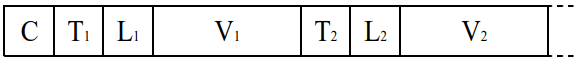
\includegraphics[scale=0.55]{trama-2.png}
\caption{\emph{Trama de controlo}}
\end{figure}

\subsection{Anexo III}
\begin{figure}[h]
	\centering
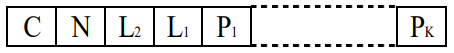
\includegraphics[scale=0.7]{trama-1.png}
\caption{\emph{Pacotes de aplicação}}
\end{figure}

\subsection{Anexo IV}
\begin{figure}[h]
	\centering
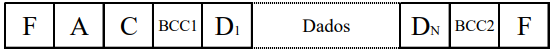
\includegraphics[scale=0.55]{trama-3.png}
\caption{\emph{Trama de informação}}
\end{figure}


\newpage
\subsection{Anexo V}
\begin{figure}[h]
	\centering
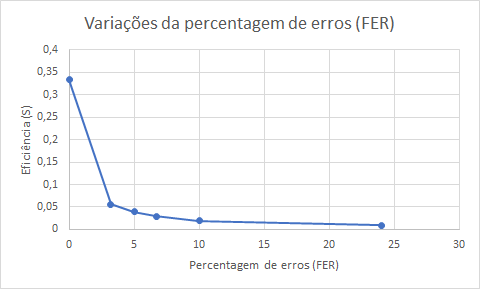
\includegraphics[scale=0.7]{fer.png}
\caption{\emph{Variação do FER}}
\end{figure}

\subsection{Anexo VI}
\begin{figure}[h]
	\centering
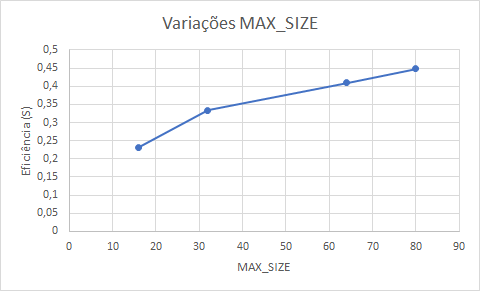
\includegraphics[scale=0.7]{maxsize.png}
\caption{\emph{Variação do max size}}
\end{figure}

\newpage
\subsection{Anexo VII}
\begin{figure}[h]
	\centering
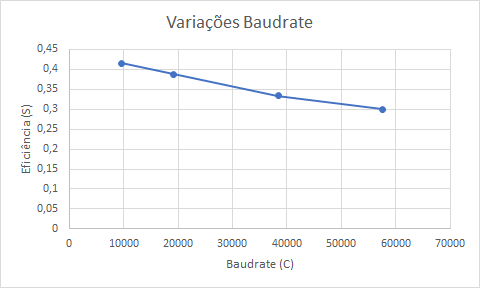
\includegraphics[scale=0.7]{baudrate.png}
\caption{\emph{Variação da baudrate}}
\end{figure}

\subsection{Anexo VIII}
\begin{figure}[h]
	\centering
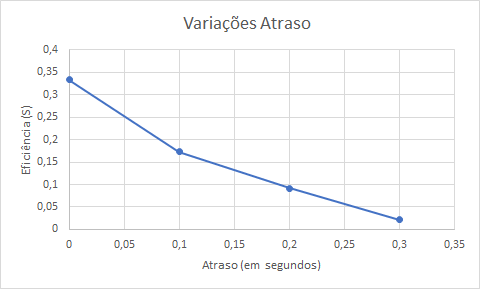
\includegraphics[scale=0.7]{atraso.png}
\caption{\emph{Variação dos atrasos de propagação}}
\end{figure}

\end{document}